\section{猜數字:幾A幾B(人猜)}

電腦選定一個沒有重複的三位數當作答案,使用者每猜一個數字,電腦會根據答案給出幾A幾B的提示。A表示位置正確的數的個數,B表示數字正確但位置錯誤的數的個數。

使用者根據提示一直猜,直到猜中為止。
\begin{figure}[H]
	\centering
	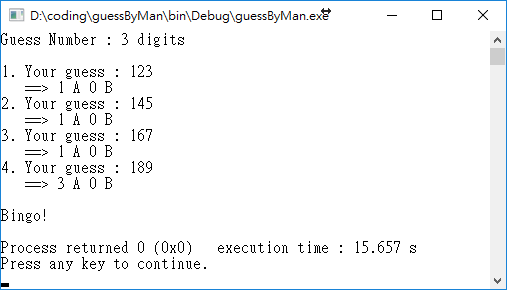
\includegraphics{fig/man}
\end{figure}
\subsection{解題思惟}

\subsubsection{程式流程:}
\begin{enumerate}
	\item 取得一個不重複的三位數。
	\item 讓使用者輸入猜的數字。
	\item 計算幾個A。
	\item 計算幾個B
	\item 若沒猜中,回到步驟2,猜中則結束程式。
\end{enumerate}

\subsubsection{函式說明:}
\begin{enumerate}
	\item int getRand3()
	
	此函數用來產生一個不重複的三位數。整數a, b, c分別是此三位數的百位、十位及個位數,一次只選定一個位數的值,每次使用$rand()\%10$來取得一個介於0-9之間的隨機亂數,若與其他位數的值相同,則重新取亂數,一直取到與其他位數不相等為止。最終取得的三位數是$(a*100+b*10+c)$。
	
	\item int countA(int guess, int ans)
	
	此函數用來計算幾個A。參數guess是使用者猜的數字,ans是答案。使用\%10分別取得guess及ans的個位數,比較兩數,若相等,則cnt++。比較完之後將guess及ans分別除以10。因為guess及ans是一個三位數,所以用for迴圈執行3次比較。最後輸出cnt即可知道猜中幾個A。
	
	\item int countB(int guess, int ans)
	
	此函數用來計算幾個B。將guess及ans的個位、十位及百位數分別存入陣列a及陣列b。使用雙重for迴圈掃描所有情況,若位置不同$(i != j)$且數字相同$(a[i] == b[j])$,則cnt++。最後輸出cnt即可知道猜中幾個B。
\end{enumerate}

\subsection{程式碼}
\begin{cppcode}
#include <iostream>
#include <cstdlib>
#include <ctime>

using namespace std;

int getRand3();
int countA(int guess, int ans);
int countB(int guess, int ans);

int main()
{
	int mynumber, yourguess, idx=1;
	cout << "Guess Number : 3 digits\n\n";
	mynumber = getRand3();
	do {
		cout << idx++ << ". Your guess : ";
		cin >> yourguess;
		int a = countA(mynumber, yourguess);
		int b = countB(mynumber, yourguess);
		cout << "   ==> " << a << " A " << b << " B" << endl;
	} while (yourguess != mynumber);
	cout << endl << "Bingo!" << endl;
	return 0;
}

int countA(int guess, int ans)
{
	int d1, d2, cnt=0;
	for (int i=0; i<3; i++) {
		d1 = guess % 10;
		d2 = ans % 10;
		if (d1==d2) cnt++;
		guess /= 10;
		ans /= 10;
	}
	return cnt;
}

int countB(int guess, int ans)
{
	int a[3], b[3], cnt=0;
	for (int i=0; i<3; i++) {
		a[i] = guess % 10;
		b[i] = ans % 10;
		guess /= 10;
		ans /= 10;
	}
	for (int i=0; i<3; i++) {
		for (int j=0; j<3; j++) {
			if (i!=j && a[i]==b[j]) cnt++;
		}
	}
	return cnt;
}

int getRand3()
{
	int a, b, c;
	srand(time(NULL));
	
	a = rand() % 10; // 0--9
	
	do {
		b = rand() % 10;
	} while (b==a);  // if b==a, re-choose b
	
	do {
		c = rand() % 10;
	} while (c==a || c==b);  // if c==a or c==b, re-choose c
	
	return a*100+b*10+c;
}
\end{cppcode}